\documentclass{article}
\usepackage[margin=1in]{geometry} 
\usepackage{amsmath,amsthm,amssymb,amsfonts, fancyhdr, color, comment, graphicx, environ, float}
\usepackage{mdframed}
\usepackage[shortlabels]{enumitem}
\usepackage{indentfirst}
\usepackage{xcolor}
\usepackage{listings}
\definecolor{mygray}{rgb}{0.8,0.8,0.8}
\lstset{%
    basicstyle=\tt,
    breaklines = true,
    backgroundcolor=\color{mygray},
}
\usepackage{hyperref}
\hypersetup{
    colorlinks=true,
    linkcolor=blue,
    filecolor=magenta,      
    urlcolor=blue,
}
\usepackage{realboxes}
\usepackage{subcaption}

\begin{document}

\title{CS 6350 Project: Final Report}

\author{Jakob Johnson, u0972673}

\maketitle

\section{Introduction}

I chose the competitive project, working on the Income Level Prediction dataset on Kaggle. As described on Kaggle, the dataset was extracted by Barry Becker from the 1994 Census database. Our task is to predict whether a person makes over \$50,000 per year given the census demographics information. 

\subsection{Dataset}

This dataset includes a training and testing dataset, with 25,000 training observations with labels and 23,842 testing observations without labels. There are 14 attributes for each observation and 'income>50k' for the training set, the label variable we are trying to predict. Some values are missing, and question marks denote those.

There are eight categorical variables; education, marital-status, native-country, occupation, race, relationship, sex, and workclass. (Figure \ref{fig:cat_vars}) 

\begin{figure}[H]
    \centering
    \begin{subfigure}{0.3\textwidth}
        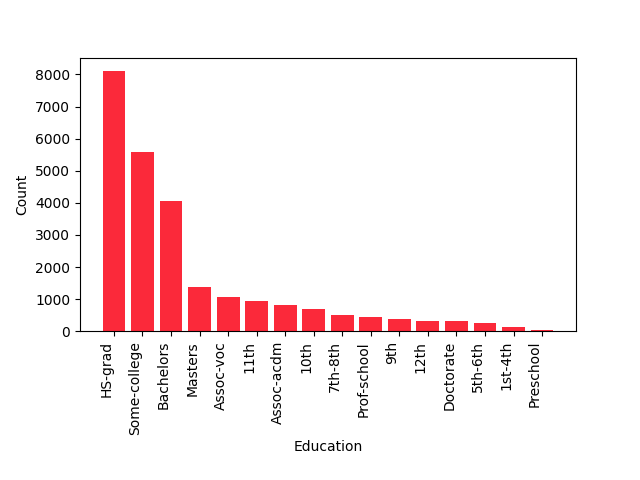
\includegraphics[width=\linewidth]{img/education.png}
    \end{subfigure}
    \begin{subfigure}{0.3\textwidth}
        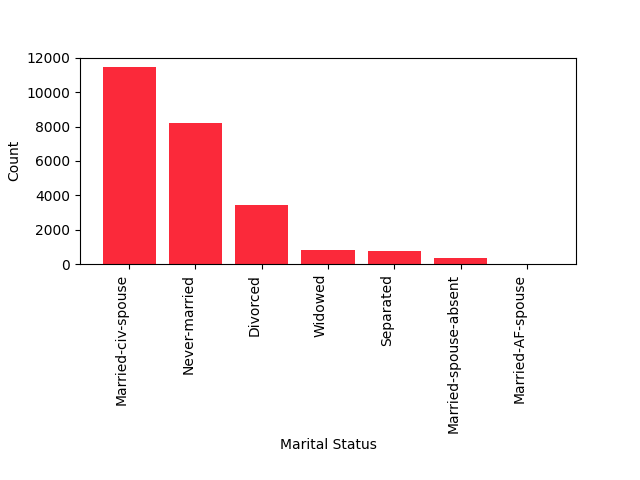
\includegraphics[width=\linewidth,]{img/marital-status.png}
    \end{subfigure}
    \begin{subfigure}{0.3\textwidth}
        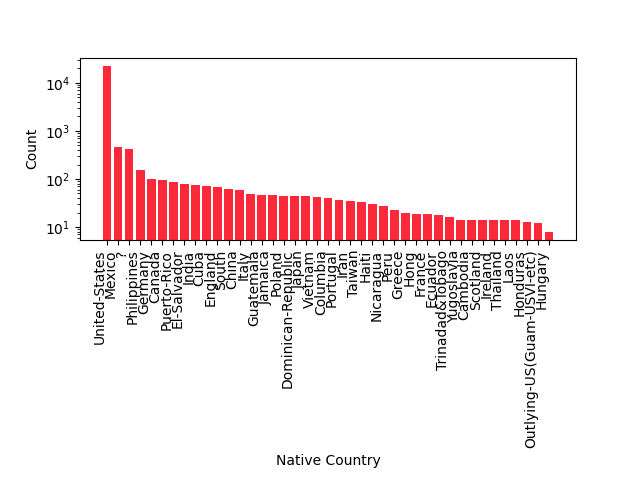
\includegraphics[width=\linewidth]{img/native-country.png}
    \end{subfigure}
    \begin{subfigure}{0.3\textwidth}
        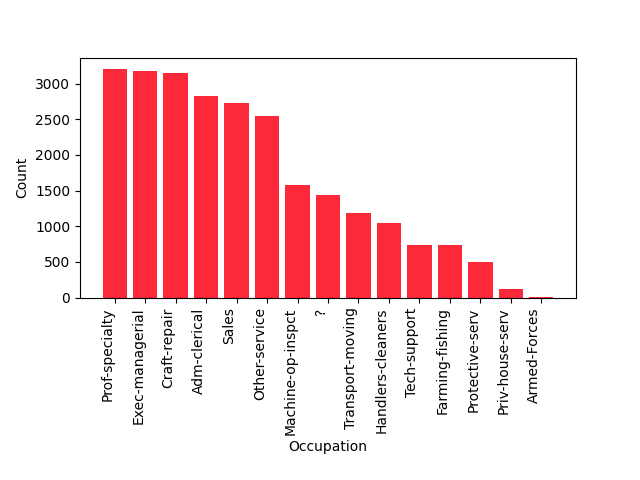
\includegraphics[width=\linewidth,]{img/occupation.png}
    \end{subfigure}
    \begin{subfigure}{0.3\textwidth}
        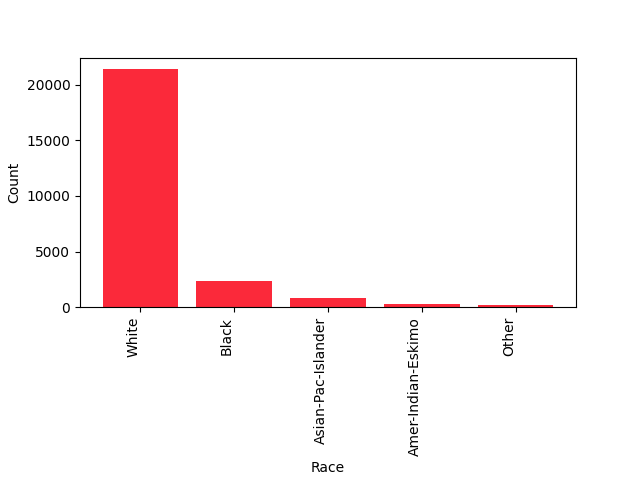
\includegraphics[width=\linewidth,]{img/race.png}
    \end{subfigure}
    \begin{subfigure}{0.3\textwidth}
        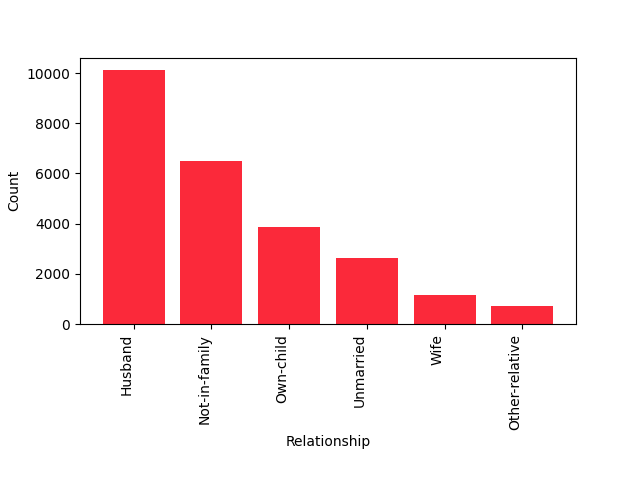
\includegraphics[width=\linewidth,]{img/relationship.png}
    \end{subfigure}
    \begin{subfigure}{0.3\textwidth}
        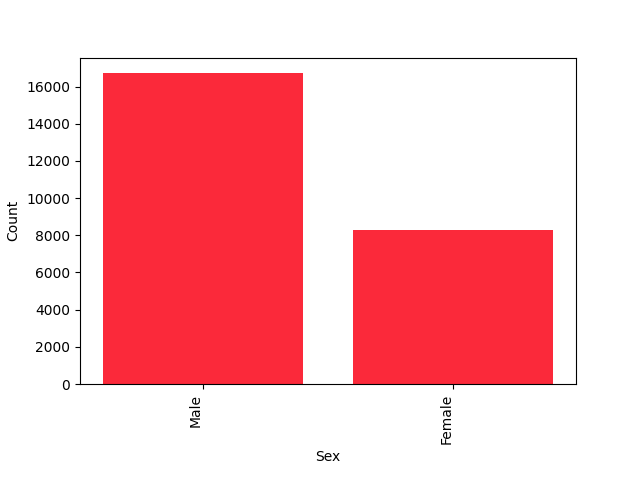
\includegraphics[width=\linewidth,]{img/sex.png}
    \end{subfigure}
    \begin{subfigure}{0.3\textwidth}
        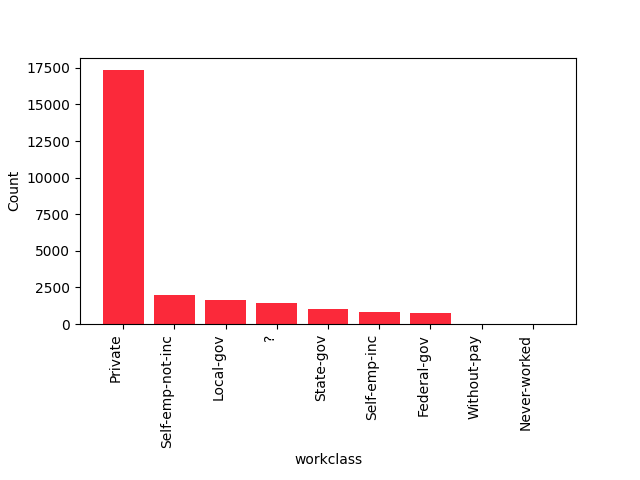
\includegraphics[width=\linewidth,]{img/workclass.png}
    \end{subfigure}

    \caption{Categorical Variables}
    \label{fig:cat_vars}
\end{figure}

There are six numeric variables; age, capital-gain, capital-loss, education-num, fnlwgt, and hours-per-week. (Figure \ref{fig:num_vars})

\begin{figure}[H]
    \centering
    \begin{subfigure}{0.3\textwidth}
        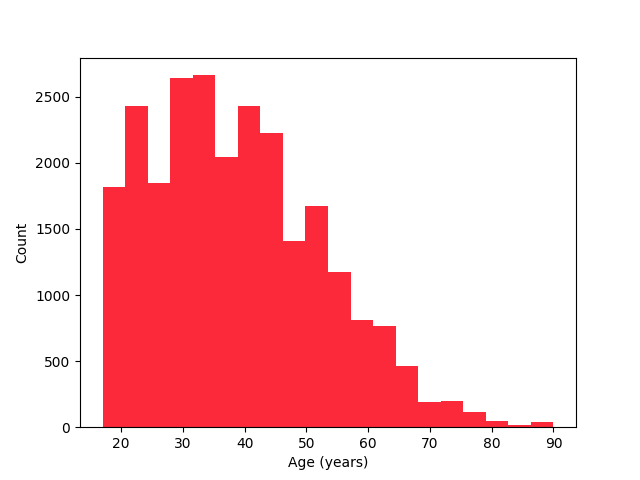
\includegraphics[width=\linewidth]{img/age.png}
    \end{subfigure}
    \begin{subfigure}{0.3\textwidth}
        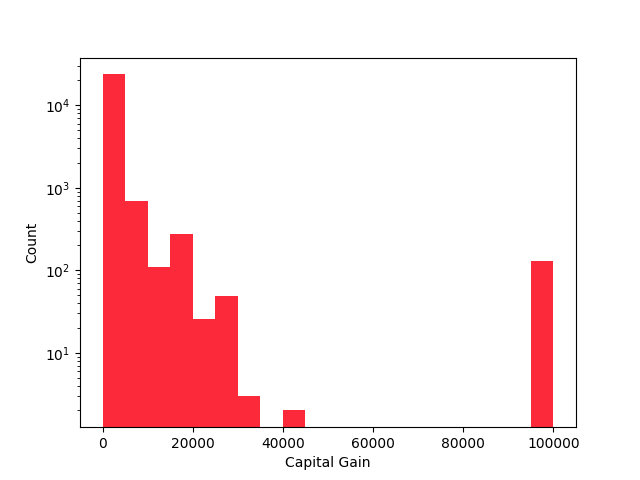
\includegraphics[width=\linewidth,]{img/capital-gain.png}
    \end{subfigure}
    \begin{subfigure}{0.3\textwidth}
        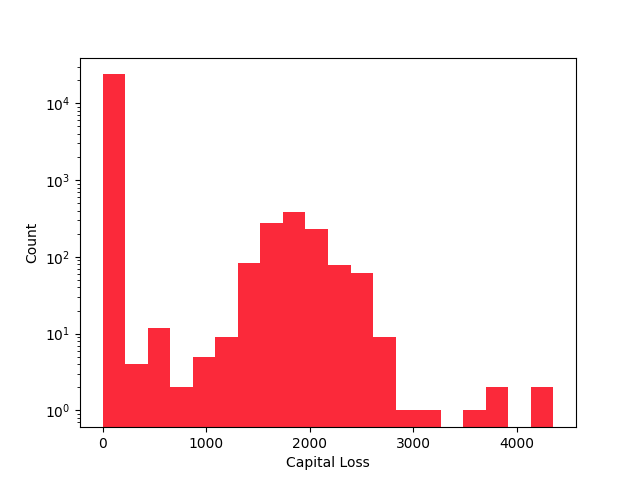
\includegraphics[width=\linewidth]{img/capital-loss.png}
    \end{subfigure}
    \begin{subfigure}{0.3\textwidth}
        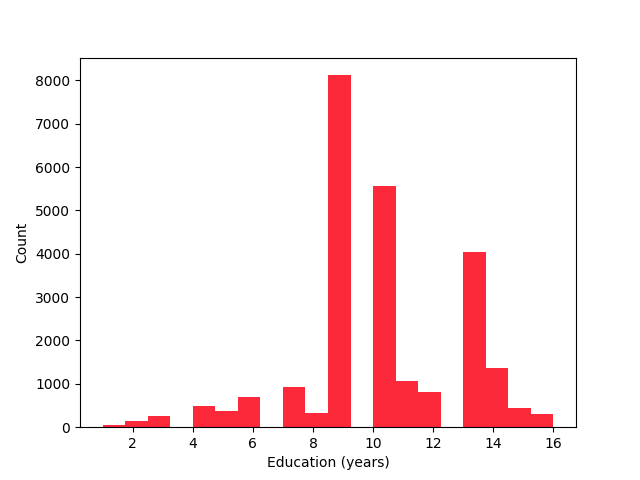
\includegraphics[width=\linewidth,]{img/education-num.png}
    \end{subfigure}
    \begin{subfigure}{0.3\textwidth}
        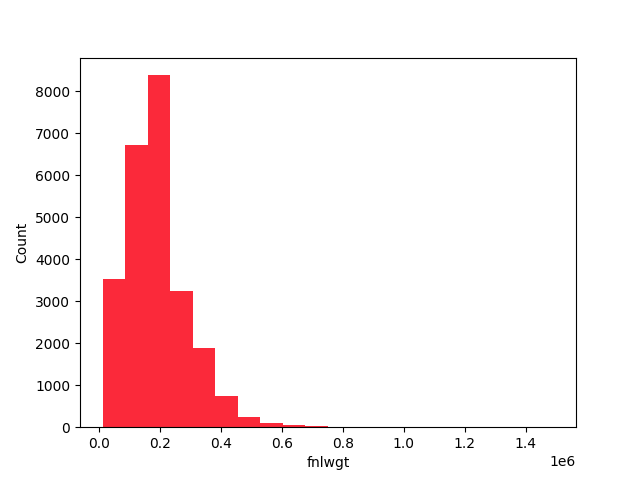
\includegraphics[width=\linewidth,]{img/fnlwgt.png}
    \end{subfigure}
    \begin{subfigure}{0.3\textwidth}
        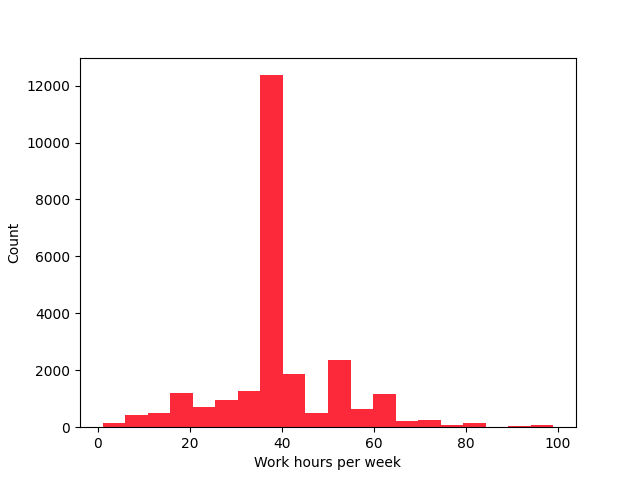
\includegraphics[width=\linewidth,]{img/hours-per-week.png}
    \end{subfigure}

    \caption{Numeric Variables}
    \label{fig:num_vars}
\end{figure}

The output label, 'income>50K', is relatively unbalanced, with about 75\% of the dataset labeled 0 and the remainder with 1. 

(plot here)

\section{Methods \& Results}

The following implementations are available on GitHub: https://github.com/jakobottar/2021-ml-project.

\subsection{Adaboost}
\
I first tried to fit the model with AdaBoost. I suspected that a simple decision tree would not do well, and AdaBoost should do at least as well as a single tree. I chose the Scikit-learn implementation AdaBoostClassifier. This implementation requires a feature array and a result array that are all numeric, so I had to read in the data with pandas and perform feature mapping to convert the string-formatted categorical variables to numeric variables that the AdaBoost classifier could read. 

After formatting the data, I wanted to determine the best number of classifiers to include in my AdaBoost model, so I ran 5-fold cross-validation on models using 1 to 750 (skipping every 10) classifiers. I stored the number of classifiers with the highest accuracy and plotted the accuracy (figure \ref{fig:adaboost}). I achieved a max training accuracy of approximately 87\%.

\begin{figure}[h]
    \centering
    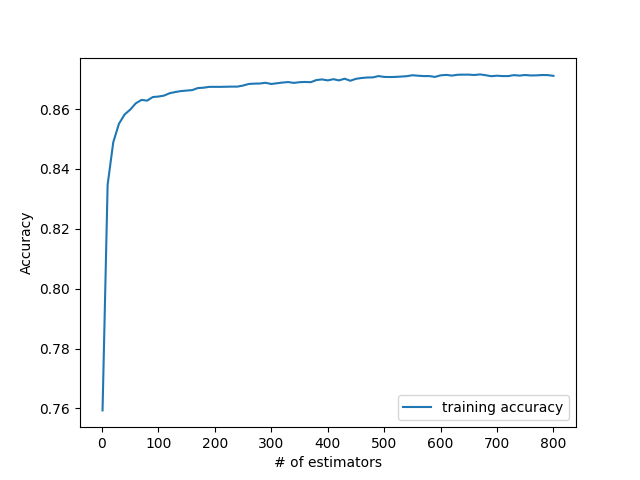
\includegraphics[width=0.4\linewidth]{img/ab_acc.png}
    \caption{Adaboost Accuracy vs Number of Classifiers}
    \label{fig:adaboost}
\end{figure}

In the end, I used 750 classifiers to train the final model using all the training data. I could potentially continue to increase the number of classifiers. Still, the model takes quite a bit of time to train at 750, and that only showed marginal gains over models using 300 and 500 estimators.

After training the model, I formatted the testing set the same way as the training set, converting categorical variables to numeric, and used the fully-trained model to predict each value's 'income>50K' attribute. Saving this as a CSV and uploading it to Kaggle showed an accuracy of 73.041\%. 

\subsection{Random Forests}

After trying AdaBoost and getting a decent result, I decided to try a similar method - Random Forests. Since Random Forests are more robust to overfitting and we got a training accuracy of 87\% and testing accuracy of only 73\%, I think the model might be overfitting too much. I again chose the Scikit-learn implementation RandomForestClassifier. Like AdaBoostClassifier, this implementation requires a feature array and a result array that are all numeric, so I had to read in the data with pandas and perform feature mapping to convert the string-formatted categorical variables to numeric variables that the Random Forest classifier could read. 

After formatting the data, I again wanted to determine the best number of classifiers to include in my Random Forest model, so I ran 5-fold cross-validation on models using 1 to 750 (skipping every 10) classifiers. I stored the number of classifiers with the highest accuracy and plotted the accuracy (figure \ref{fig:rf}). We achieved a max training accuracy of approximately 86\%, slightly lower than AdaBoost. 

\begin{figure}[h]
    \centering
    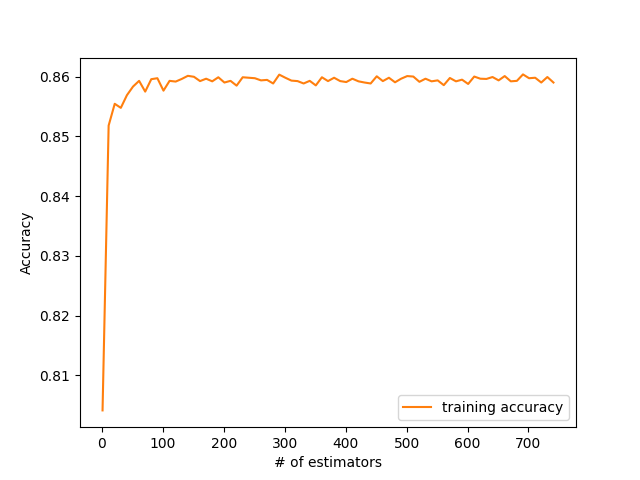
\includegraphics[width=0.4\linewidth]{img/rf_acc.png}
    \caption{Random Forest Accuracy vs Number of Classifiers}
    \label{fig:rf}
\end{figure}

In the end, I again used 750 classifiers to train the final model using all the training data.

After training the model, I formatted the testing set the same way as the training set, converting categorical variables to numeric, and used the fully-trained model to predict each value's 'income>50K' attribute. Saving this as a CSV and uploading it to Kaggle showed an accuracy of 77.197\%, slightly higher than that of AdaBoost, confirming my hypothesis that the AdaBoost model was overfitting and Random Forest's robustness to that would lead to a higher testing accuracy.

\subsection{Support Vector Machines}

As with the previous methods, I needed to convert the dataset from categorical string variables to numeric ones. The first iteration of my SVM implementation used a radial basis function kernel and no class weights. This version had a training accuracy of 78\% and a testing accuracy in Kaggle of 74\%. After analyzing the dataset and realizing how significantly it was unbalanced, I added sample weights of 0.25 to class 0 and 0.75 to class 1. This increased the training accuracy to 79.6\% and the Kaggle testing accuracy to 82\%, the highest so far by a wide margin. 

After this realization, I went back and retooled my previous methods to take advantage of class weights. They all improved in training accuracy but did not significantly improve testing accuracy. 

Finally, I tried all the available kernel functions; linear, polynomial, radial basis, and sigmoid. The polynomial kernel gave a slightly higher training accuracy than the radial basis but not a higher testing accuracy. Sigmoid and Linear kernels performed poorly. 

\subsection{Neural Nets}

Neural Nets are where I spent most of my time, as I anticipated that they would give me the best results, and they also have the most significant need for tuning and optimization. 

My implementation was based on on my neural net code and architectures from Homework 5, using a similar custom dataset and training functions. I tried two different methods of encoding the categorical variables for the dataset. One method converted category labels to integers. I also tried a method using one-hot encoding, making a column for each factor of the variable. This second method generated a much larger vector for training, 1x106 instead of 1x14. This larger training set made the net train significantly slower but did not considerably change the training or testing accuracy.

\begin{figure}[h]
    \centering
    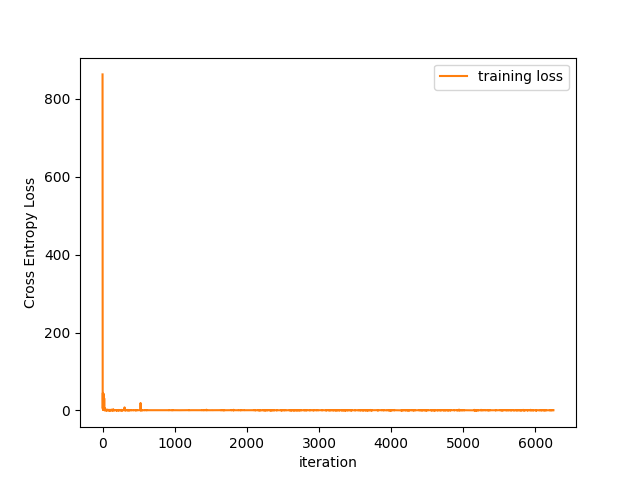
\includegraphics[width=0.4\linewidth]{img/nn_loss.png}
    \caption{Neural Net Training Loss - Final Version}
    \label{fig:nn}
\end{figure}

For the neural net architecture, I decided on one input layer, 11 50-wide connected body layers, and a two-node output layer for a total of 13 layers. I chose the two output nodes to use CrossEntropyLoss and softmax during prediction as is the norm for classification problems. At first, I used a loop to check many different combinations of body layer widths and network depths, settling on this architecture as it performed the best. 

Initially during training, my network would converge to an all-zeros prediction, with an accuracy of exactly 75.94\%, the fraction of zeros in the training dataset. This would have given an abysmal testing accuracy. To improve it, I changed optimizers to the Adam and AdamW optimizer, with AdamW at its default 1E-3 learning rate performing the best. Also in an effort to perturb the model away from its nonoptimal local minimum, I changed from ReLU activation functions to LeakyReLU ones.  

Even after all of these tweaks, I could never break an 80\% training accuracy. The models also had a very poor testing accuracy of 62\% at their peak, showing that they were massively overfitting the data. 

\subsection{Naive Bayes and Logistic Regression}
I briefly tried implementing Naive Bayes and Logistic Regression classifiers. Their initial testing accuracies were significantly below that of SVMs and Random Forests so I did not pursue these methods further. Perhaps these could be tuned to perform well in the future, but I did not have enough time. 

\subsection{Gradient Boosting Machines}

Gradient Boosting Machines were a method I saw mentioned in the Scikit Learn documentation and I decided to try it as a final method, using the sklearn GradientBoostingClassifier implementation. I did the same categorical data handling as in the other Sklearn methods. After trying a range of different numbers of estimators in the ensemble method, I trained the model on the whole training dataset, using sample weights to achieve a balanced class weight scheme. It achieved a maximum training accuracy of 87.56\% which was the highest recorded so far, and a testing accuracy of 82.88\% which was also the best so far. I briefly tried tuning some paramemters but nothing was able to improve the accuracy. 

\begin{figure}[h]
    \centering
    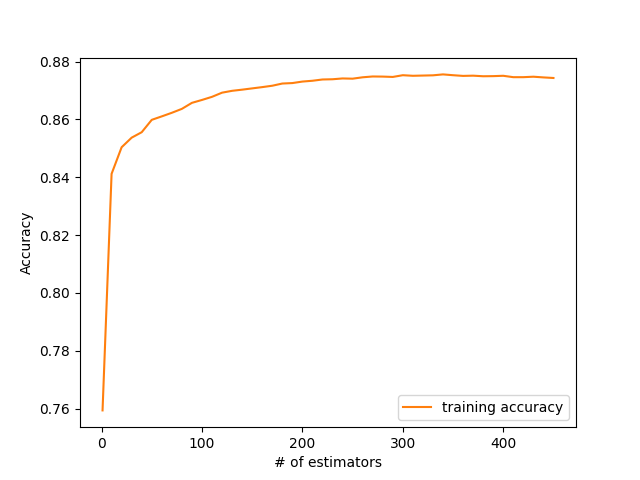
\includegraphics[width=0.4\linewidth]{img/gbm_acc.png}
    \caption{Gradient Boosting Classifier Accuracy vs Number of Classifiers}
    \label{fig:gbm}
\end{figure}

\section{Conclusion}

I achieved a pretty good maximum score of 82.88\% using Gradient Boosting Machines, and explored many different models with different approaches. Figure \ref{fig:overall_acc} shows all the training and testing accuracies of the different models.

\begin{figure}[h]
    \centering
    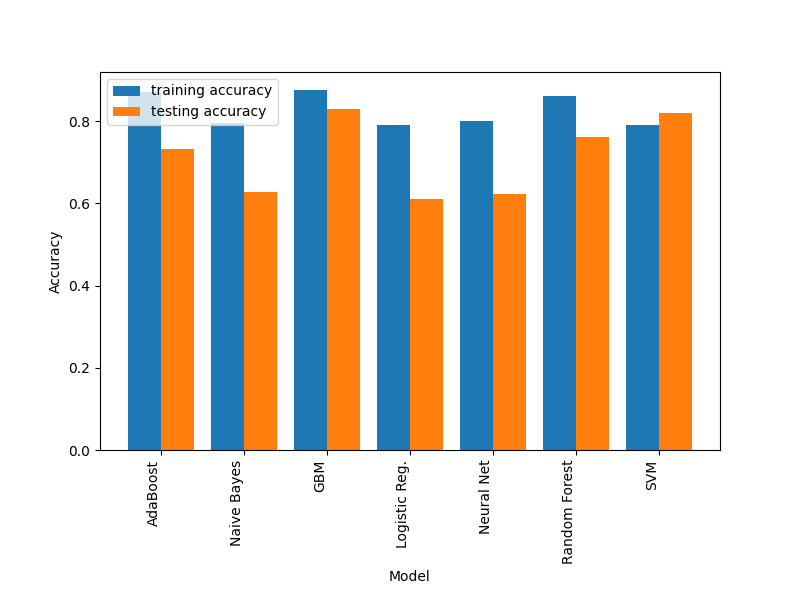
\includegraphics[width=0.6\linewidth]{img/results.png}
    \caption{Accuracy Comparison of different models}
    \label{fig:overall_acc}
\end{figure}

The ensemble methods did fairly well, but the difference in training and testing error shows they often overfit the data. The others did not seem to be properly modeling the data, with low training and very low testing accuracies. I am dissapointed in the neural net results, I still think that I could have gotten much higher accuracy with the neural net model, but it needs significantly more tuning and probably a very different architecture. 

\subsection{Future Work}
If I had additional time I would try more neural net architectures and hyperparameters. Briefly talking to other students, they had significantly better results than me with the neural net. I could also take a more statistical approach and do some correlation analysis of the variables and potentially create additional variables out of combinations of the existing ones. I would also do more research on how to handle unbalanced datasets like this one.


\end{document}
